\documentclass[11pt,a4j]{jreport}

\usepackage{comment}
\usepackage{float}
\usepackage{color}
\usepackage{multicol}
\usepackage{multirow}
\usepackage[dvipdfmx]{pict2e}
\usepackage{wrapfig}
\usepackage{graphicx}
\usepackage{bm}
\usepackage{url}
\usepackage{underscore}
\usepackage{colortbl}
\usepackage{tabularx}
\usepackage{fancyhdr}
\usepackage{ulem}
\usepackage{cite}
\usepackage{amsmath,amssymb,amsfonts}
\usepackage{algorithmic}
\usepackage{textcomp}
\usepackage{xcolor}
\usepackage[ipaex]{pxchfon}
\usepackage{pdfpages}
\usepackage{subcaption}
\usepackage{array}
\usepackage{adjustbox}
\usepackage{lipsum}

\usepackage[number-unit-product=~]{siunitx}

\usepackage[top=30truemm,bottom=30truemm,left=25truemm,right=25truemm]{geometry}

\renewcommand{\arraystretch}{1.2}

\begin{document}

\chapter{演奏実験}

%=====================================================================================

\section{実験の概要}
反射音の到来方向が合唱者の演奏時の主観印象評価に与える影響について検討するため、第4章で生成した音場を用いて
声楽カルテットによる演奏実験を行った。基準音場での演奏ののちに方向特性を変化させた音場AからDのうちいずれかの
音場での演奏を行い、その印象の変化について回答を得る試行をAからDのすべての音場について繰り返すことで、反射音の
到来方向特性を変化させたときの演奏時の印象の変化を調べた。

演奏実験はソプラノ、アルト、テノール、バスによる4人1組の混声四部の四重奏にて行った。被験者は合唱経験者31名
(ソプラノ・アルト・バス8人、テノール7人。うち声楽経験者9名)であり、8組の実験グループを作成した。なお、
実験グループのうち一つのグループでテノールに欠員が生じたため、そのグループにおいては筆者がテノールとして
演奏に参加した。

実験には平易な日本語の混声四部合唱曲として「ふるさと」の一番を用いた。音場AからDの提示順序はランダムとした。
並び順は一般的な混声四部のカルテットと同様に、舞台下手側として想定した方からソプラノ、アルト、テノール、バスの
順とした。演奏実験の様子を図\ref{fig:演奏実験の様子}に示す。

\vspace{1\baselineskip}

\begin{figure}[H]
  \centering
  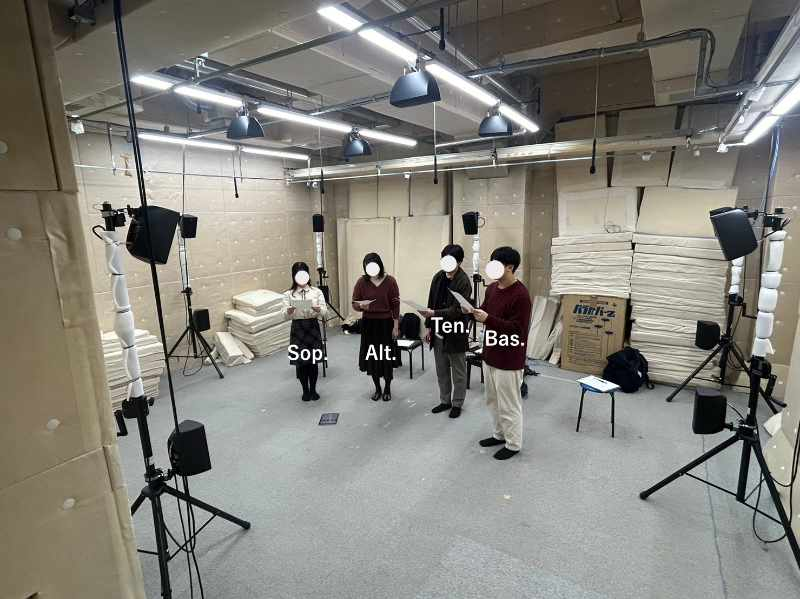
\includegraphics[width=0.7\linewidth]{images/subjectiveExp/chorusExpLowQ.jpg}
  \caption{演奏実験の様子}
  \label{fig:演奏実験の様子}
\end{figure}

%=====================================================================================
\clearpage

\section{手順}

被験者は基準音場での演奏と音場AからDのいずれか一つの音場での演奏ののち、評定尺度法による段階評価および
自由記述による音場の印象の評価を行い、これを音場AからDすべてについて終えるまで繰り返した。実験全体の流れを
図\ref{tab:実験全体の流れ}に、実験1条件あたりの流れを図\ref{tab:実験1条件あたりの流れ}に示す。

(手順の決定方法について記述。教示の内容、実験における時間の使い方について柔軟に対処したこと、求めた完成度の基準、
立ち位置に関しての取り決め、演奏の始め方)


評定尺度は-3から3までの7段階評価とし、
評定項目は音場の印象に関する3項目、空間の印象に関する4項目、演奏の印象に関する4項目、総合的な印象に関する2項目の
13項目とした。段階評価に用いた評価項目および評価尺度を表\ref{tab:段階評価の評価項目および評定尺度}の通りとした。
すべての条件での演奏および評価が終了した後に、自由記述による全体を通した印象の評価を行った。

(評価項目および評価尺度の決定の仕方、検討したことを記述)



\clearpage

\begin{table}[H]
  \centering
  \caption{実験全体の流れ}
  \label{tab:実験全体の流れ}

  \begingroup
  \renewcommand{\arraystretch}{1.2}

  \begin{tabular}{|c|c|}
    時間 & 内容 \\
    \hline
    0:00〜0:10 & 説明、同意書およびフェイスシートの記入 \\
    0:10〜0:25 & ウォーミングアップ・音取り \\
    0:25〜0:30 & 1回目の演奏実験(基準音場→AからDのうち一つの音場)と評価 \\
    0:30〜0:35 & 2回目の演奏実験(基準音場→AからDのうち一つの音場)と評価 \\
    0:35〜0:40 & 3回目の演奏実験(基準音場→AからDのうち一つの音場)と評価 \\
    0:40〜0:45 & 4回目の演奏実験(基準音場→AからDのうち一つの音場)と評価 \\
    0:45〜0:50 & 全体を通した評価\\
    0:50〜0:55 & 回答用紙を回収して終了 \\
  \end{tabular}
  \endgroup
\end{table}

\vspace{1\baselineskip}

\begin{table}[H]
  \centering
  \caption{実験1条件あたりの流れ}
  \label{tab:実験1条件あたりの流れ}

  \begingroup
  \renewcommand{\arraystretch}{1.2}

  \begin{tabular}{|m{3cm}|m{3cm}|m{9cm}|}
    \multicolumn{1}{|c|}{基準音場で演奏} &
    \begin{tabular}{c}音場A〜Dの\\いずれかで演奏
    \end{tabular}
    & \multicolumn{1}{c|}{響きの印象の変化を評価} \\
    \hline
    \multicolumn{1}{|c|}{1分} & \multicolumn{1}{c|}{1分} & \multicolumn{1}{c|}{3分} \\ 
  \end{tabular}
  \endgroup
\end{table}

\vspace{1\baselineskip}

\begin{table}[H]
  \centering
  \caption{段階評価の評価項目および評定尺度}
  \label{tab:段階評価の評価項目および評定尺度}

  \begingroup
  \renewcommand{\arraystretch}{1.2}
  \begin{tabular}{c|c|c}
    & 評価項目 & 評定尺度($-3$ 〜 $3$の7段階) \\
    \hline \hline

    \multirow{3}{*}{音場の印象} & 響きが増えたか & 減った / 増えた \\
    \cline{2-3}
    & 自分の音の聴きやすさ & \multirow{2}{*}{聴きやすくなった / 聴きにくくなった}\\
    \cline{2-2}
    & 他人の音の聴きやすさ & \\
    \hline \hline

    \multirow{4}{*}{空間の印象} & 空間の広がり & 狭くなった / 広くなった \\
    \cline{2-3}
    & 客席全体に届く感じ & \multirow{3}{*}{減った / 増えた} \\
    \cline{2-2}
    & 自分に音が返る感じ & \\
    \cline{2-2}
    & 音に包まれる感じ & \\
    \hline \hline

    \multirow{4}{*}{演奏の印象} & 疲れ感 & 疲れやすくなった / 疲れにくくなった \\
    \cline{2-3}
    & 強弱のつけやすさ & つけやすくなった / つけにくくなった \\
    \cline{2-3}
    & アンサンブルのしやすさ & しにくくなった / しやすくなった\\
    \cline{2-3}
    & 音が溶け合う感じ & 減った / 増えた \\
    \hline \hline

    \multirow{2}{*}{総合的な印象} & 演奏がうまくいったか & うまくいかなかった / うまくいった \\
    \cline{2-3}
    & 演奏のしやすさ & しにくくなった / しやすくなった \\
    \hline

  \end{tabular}
  \endgroup
\end{table}

%=====================================================================================
\clearpage
\section{結果と考察}

\subsection{段階評価の結果と考察}

\subsection*{全被験者の評価}
  評定尺度法による段階評価における全被験者(N = 31)の評点平均と標準偏差(エラーバー)を図\ref{fig:評定尺度法による段階評価の平均値と標準偏差}に示す。
  また段階評価の各項目について「平均値が0に等しい」ことを帰無仮説とするt検定(両側検定)を行なったところ、
  いくつかの項目で有意差が検出されたため、0.01 ≦ p < 0.05 の項目を*、p < 0.01 の項目を**として
  検定結果を図中に併せて示す。

  まず、響きの印象についての三項目のうち、「響きが増えたか」では音場A、音場C、音場Dで基準音場よりも評価が
  高くなる傾向が見られた。前章の図\ref{fig:実験音場の残響時間}に示すように、生成した実験音場では基準音場に対してわずかに
  残響時間が増加しており、この残響時間の増加が評価に影響を与えた可能性があるものの、伸長した残響時間は有意差の
  検出されていない音場Bで最も長くなっているため、残響時間の伸長のみではこの結果を説明することができない。
  音場Bは後方からの初期反射音を増強した音場で、後壁からの初期反射音供給が多い現実の音場を模している基準音場と
  似通った方向特性となっているが、音場A、C、Dは方向特性の変化が音場Bよりも大きく、反射音到来方向の変化が
  響きの増加感に影響を与えている可能性が示唆される。

  「自分が発した音の聴きやすさ」については基準音場に対する有意差は検出されなかったが、「他人が発した音の
  聴きやすさ」については音場Cで評価が高くなった。

  全体の傾向として、平均値は1以下と小さい値となった。特に、初期反射音の方向特性に変化を与えた音場Aと音場Bでは
  ほとんどすべての評価項目で0.5以下の値となった。初期反射音は$\SI{0.1}{\second}$以内というごく短い時間に到来する
  ため、主観印象への影響は音色の変化として生じることが多く、大きな音色の変化を伴わない方向特性の変化が
  知覚されにくかったためと考えられる。
  
  また、全体に標準偏差は1以上と大きい値を取っており、これは個人間での音場の評価のばらつきが大きいことを表しているが、
  演奏の印象に関する4項目については標準偏差が比較的小さく、平均値が全体の評価の傾向をあ比較的よく表していると
  考えられる。「疲れ感」の評価については、平均値はほぼ0であり、方向特性による影響はほとんどないと考えられ、
  一方で「強弱のつけやすさ」「アンサンブルのしやすさ」「音が溶け合う感じ」の評価については、後期反射音の前方の反射音を強めた
  音場Cの値が大きい。音場Cは他の評価項目でも比較的高い平均値となっており、前方からの後期反射音の供給によって演奏時の
  印象を向上させることができる可能性があると考えられる。
  
  一方で、響きの印象に関する項目と空間の印象に関する項目について、特に「響きが増えたか」「空間の広がり」「自分に音が返る感じ」
  「音に包まれる感じ」は標準偏差が大きく、平均値が全体の評価の傾向を代表しているとは言えない。これらの評価項目について、
  全被験者の回答の散布図を図\ref{fig:響きが増えたかの散布図}から\ref{fig:音に包まれる感じの散布図}に示す。図中の破線は
  各評価項目について-2または-3を低評価、-1から1を中間評価、2または3を高評価としたときの、評価に応じた被験者の組を示している。
  
  「響きが増えたか」「空間の広がり」「自分に音が返る感じ」「音に包まれる感じ」の評価項目の被験者の分布について、初期反射音に
  方向特性に変化を与えた音場Aと音場Bでは、どちらの評価も低評価から高評価まで広く散らばっているのに対し、後期反射音に方向特性を与えた音場Cと
  音場Dの分布では、少なくとも一方を高く評価した被験者が多い傾向が見られる。このことから、後期反射音の方向特性に変化を与えることで、
  響きの印象や空間の印象を向上させることができる可能性があることが示唆される。
  

  \begin{figure}[H]
    \centering
    
    \begin{minipage}{1\linewidth}
      \centering
      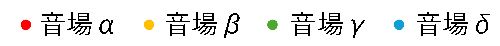
\includegraphics[scale=.55]{images/subjectiveExp/statisticAnalysis/legend.pdf}
      \label{fig:段階評価の凡例}
    \end{minipage}

    \vspace{1\baselineskip}

    \begin{minipage}{1\linewidth}
      \centering
      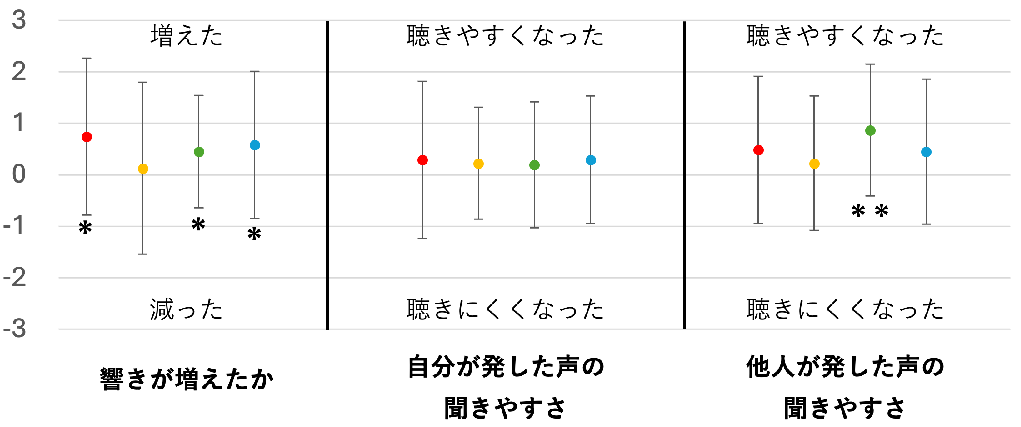
\includegraphics[scale=.55]{images/subjectiveExp/statisticAnalysis/01reverb_a.pdf}
      \caption*{響きの印象}
      \label{fig:響きの印象}
    \end{minipage}
    \\
    \vspace{1\baselineskip}
    \begin{minipage}{1\linewidth}
      \centering
      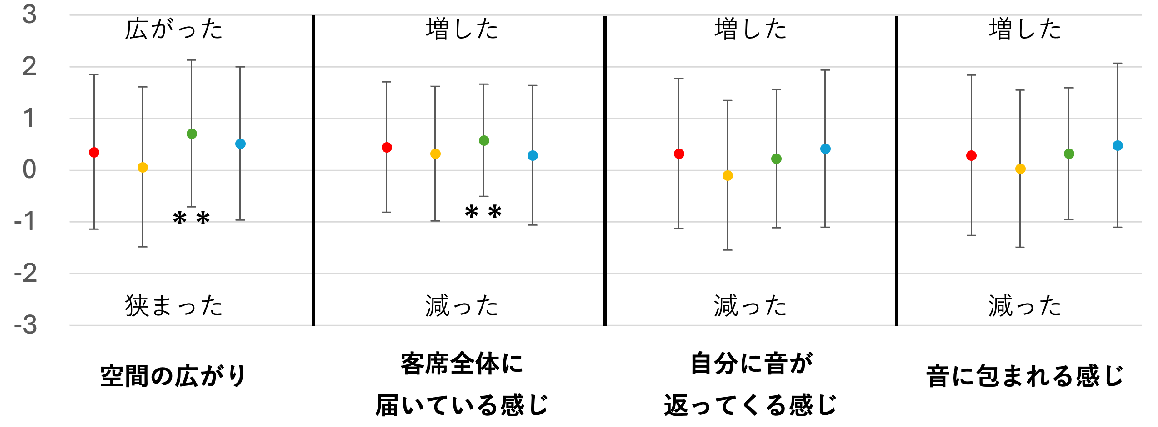
\includegraphics[scale=.55]{images/subjectiveExp/statisticAnalysis/02space_a.pdf}
      \caption*{空間の印象}
      \label{fig:空間の印象}
    \end{minipage}
    \\
    \vspace{1\baselineskip}
    \begin{minipage}{1\linewidth}
      \centering
      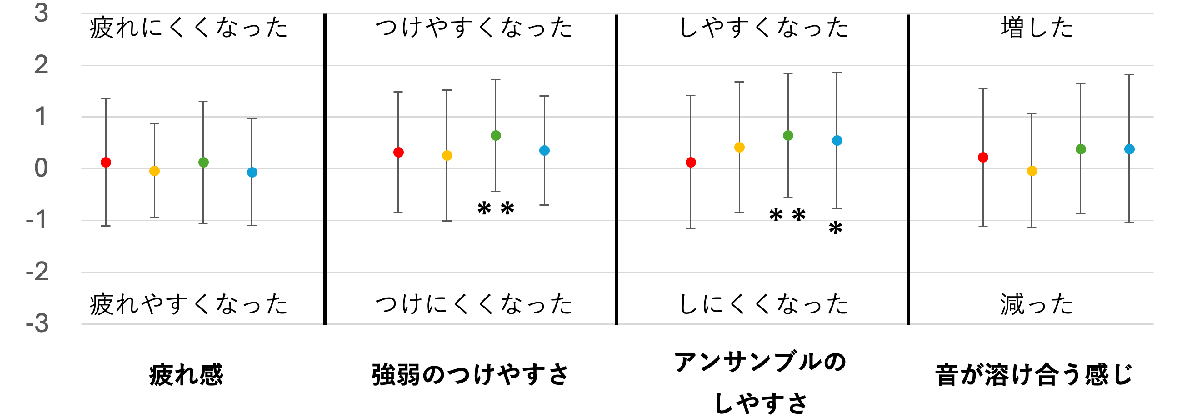
\includegraphics[scale=.55]{images/subjectiveExp/statisticAnalysis/03performance_a.pdf}
      \caption*{演奏の印象}
      \label{fig:演奏の印象}
    \end{minipage}
    \\
    \vspace{1\baselineskip}
    \begin{minipage}{1\linewidth}
      \centering
      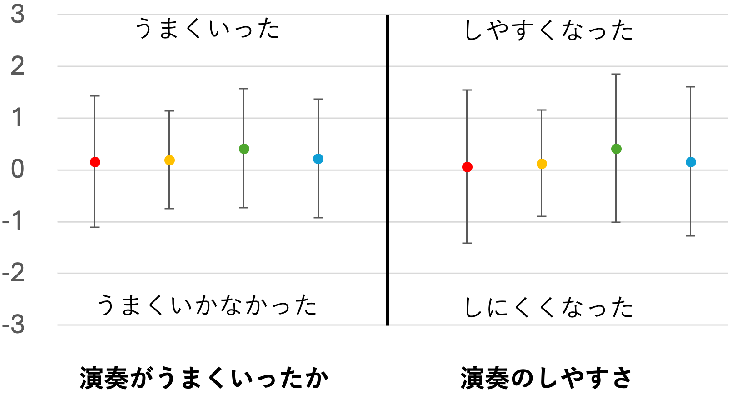
\includegraphics[scale=.55]{images/subjectiveExp/statisticAnalysis/04overall_a.pdf}
      \caption*{総合的な評価}
      \label{fig:総合的な評価}
    \end{minipage}
    

    \caption{評定尺度法による段階評価の平均値と標準偏差(* p < 0.05 \hspace{5mm} ** p < 0.01)}
    \label{fig:評定尺度法による段階評価の平均値と標準偏差}
  \end{figure}


  \clearpage

  \subsection*{パートによる評価の違い}
  本実験では、演奏時の条件を現実的な条件に近いものとするため、標準的な混声四部のカルテットの並び順に倣い、舞台下手側と想定したから
  ソプラノ・アルト・テノール・バスの順の並びとした。演奏者のパートにより、自身の音域や立ち位置、アンサンブルにおける音楽上の役割が
  異なっているため、パートによって評価に異なった傾向が現れる可能性がある。そこで、パートによる評価の違いを調べるため、パートごとの
  評点平均と標準偏差を計算した。この結果を図\ref{fig:パートごとの平均値と標準偏差A}から図\ref{fig:パートごとの平均値と標準偏差D}に
  各音場ごとに示す。
  段階評価の各項目について「平均値が0に等しい」ことを帰無仮説とするt検定(両側検定)を行なったところ、
  いくつかの項目で有意差が検出された。また、同一の音場での同一の評定項目に対するすべてのパートの組み合わせについて、
  「評定平均が等しい」ことを帰無仮説とするステューデントのt検定を行なったところ、いくつかの項目で有意差が検出された。
  これらの検定結果について、0.01 ≦ p < 0.05 の項目を*、p < 0.01 の項目を**として図中に併せて示す。

  \subsubsection*{響きの印象に関する評価}
  なんとかかんとか

  \newpage
  \begin{figure}[H]
    \centering
    
    \begin{minipage}{1\linewidth}
      \centering
      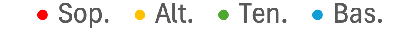
\includegraphics[scale=.55]{images/subjectiveExp/statisticAnalysis/part_legend.pdf}
    \end{minipage}
    \vspace{.5\baselineskip}

    \begin{minipage}{1\linewidth}
      \centering
      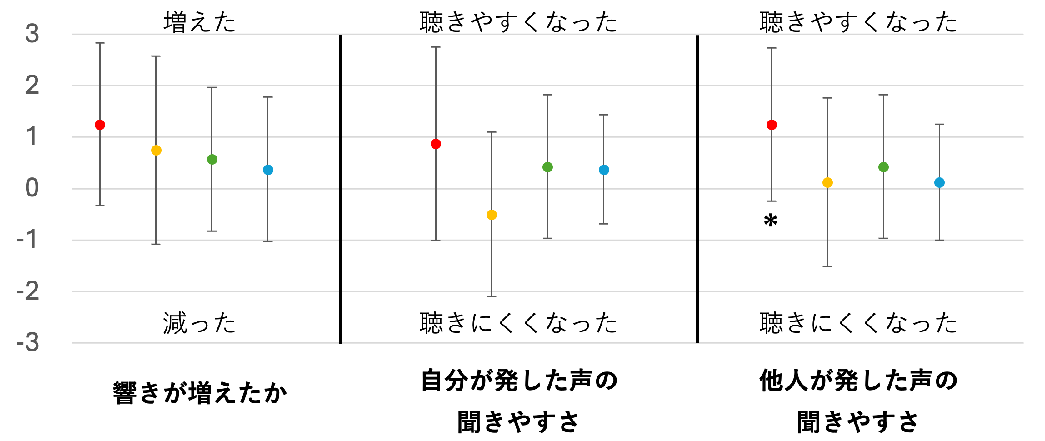
\includegraphics[scale=.55]{images/subjectiveExp/statisticAnalysis/part_reverb_a.pdf}
      \caption*{音場A}
      \label{fig:響きの印象A}
    \end{minipage}
    \\
    \vspace{1\baselineskip}
    \begin{minipage}{1\linewidth}
      \centering
      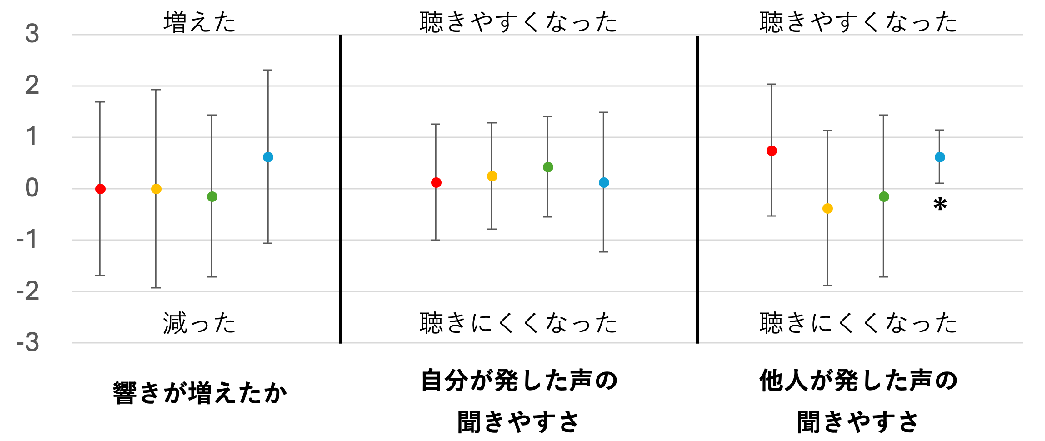
\includegraphics[scale=.55]{images/subjectiveExp/statisticAnalysis/part_reverb_b.pdf}
      \caption*{音場B}
      \label{fig:響きの印象B}
    \end{minipage}
    \\
    \vspace{1\baselineskip}
    \begin{minipage}{1\linewidth}
      \centering
      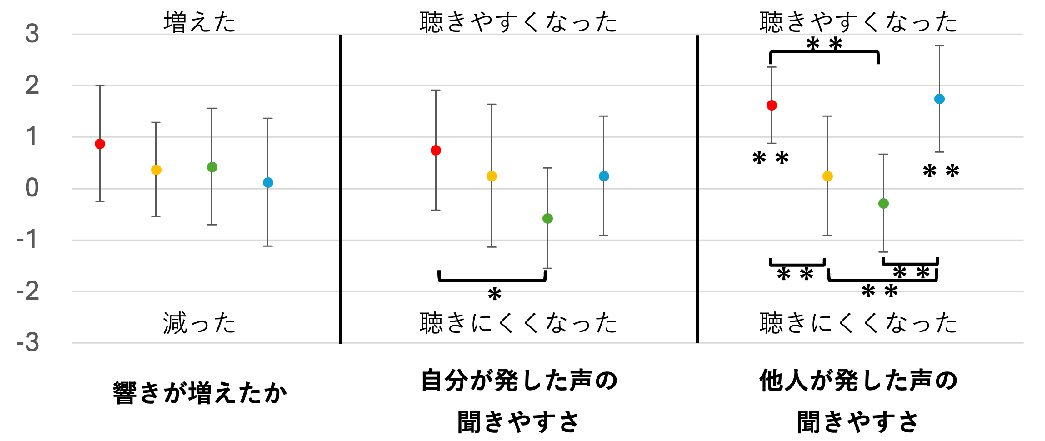
\includegraphics[scale=.55]{images/subjectiveExp/statisticAnalysis/part_reverb_c.pdf}
      \caption*{音場C}
      \label{fig:響きの印象C}
    \end{minipage}
    \\
    \vspace{1\baselineskip}
    \begin{minipage}{1\linewidth}
      \centering
      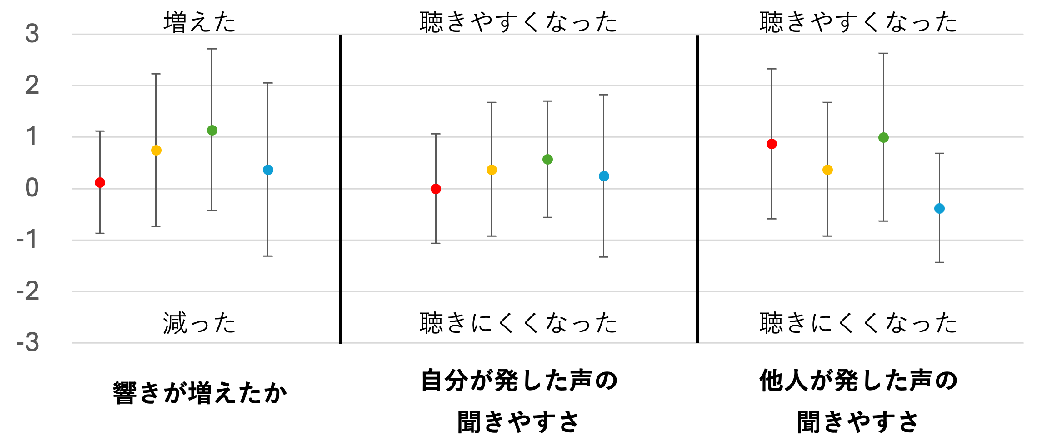
\includegraphics[scale=.55]{images/subjectiveExp/statisticAnalysis/part_reverb_d.pdf}
      \caption*{音場D}
      \label{fig:響きの印象D}
    \end{minipage}
    
    \caption{パートごとの響きの印象に関する評価}
    \label{fig:パートごとの響きの印象に関する評価}
  \end{figure}


  \clearpage
  \subsubsection*{空間の印象に関する評価}
  なんとかかんとか

  \subsubsection*{演奏の印象に関する評価}
  なんとかかんとか

  パートごとの空間の印象に関する評価とパートごとの演奏の印象に関する評価について

  パートごとの空間の印象に関する評価とパートごとの演奏の印象に関する評価について

  パートごとの空間の印象に関する評価とパートごとの演奏の印象に関する評価について

  パートごとの空間の印象に関する評価とパートごとの演奏の印象に関する評価について

  パートごとの空間の印象に関する評価とパートごとの演奏の印象に関する評価について

  パートごとの空間の印象に関する評価とパートごとの演奏の印象に関する評価について

  パートごとの空間の印象に関する評価とパートごとの演奏の印象に関する評価について

  パートごとの空間の印象に関する評価とパートごとの演奏の印象に関する評価について

  パートごとの空間の印象に関する評価とパートごとの演奏の印象に関する評価について

  パートごとの空間の印象に関する評価とパートごとの演奏の印象に関する評価について

  パートごとの空間の印象に関する評価とパートごとの演奏の印象に関する評価について

  パートごとの空間の印象に関する評価とパートごとの演奏の印象に関する評価について

  
  \newpage
  \begin{figure}[H]
    \centering
    
    \begin{minipage}{1\linewidth}
      \centering
      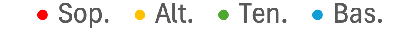
\includegraphics[scale=.55]{images/subjectiveExp/statisticAnalysis/part_legend.pdf}
    \end{minipage}
    \vspace{.5\baselineskip}

    \begin{minipage}{1\linewidth}
      \centering
      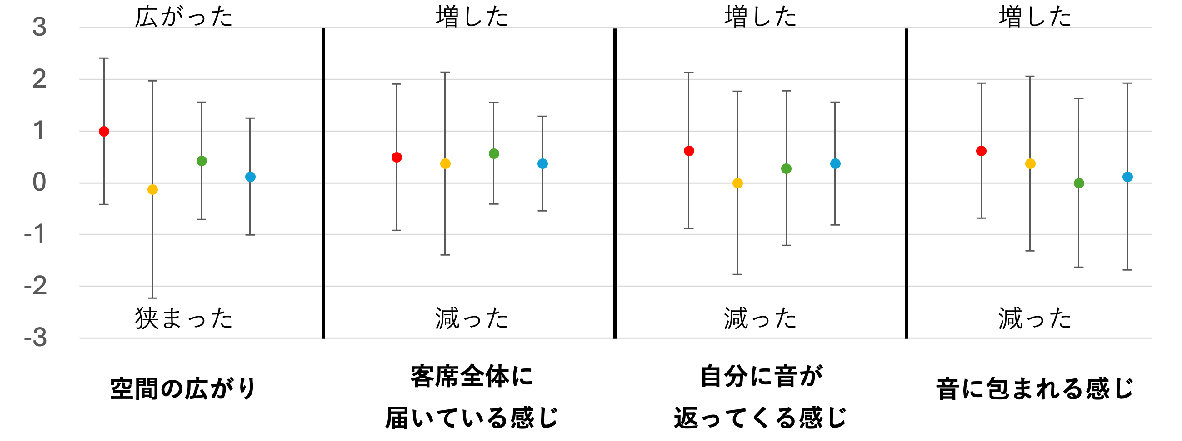
\includegraphics[scale=.55]{images/subjectiveExp/statisticAnalysis/part_space_a.pdf}
      \caption*{音場A}
      \label{fig:空間の印象A}
    \end{minipage}
    \\
    \vspace{1\baselineskip}
    \begin{minipage}{1\linewidth}
      \centering
      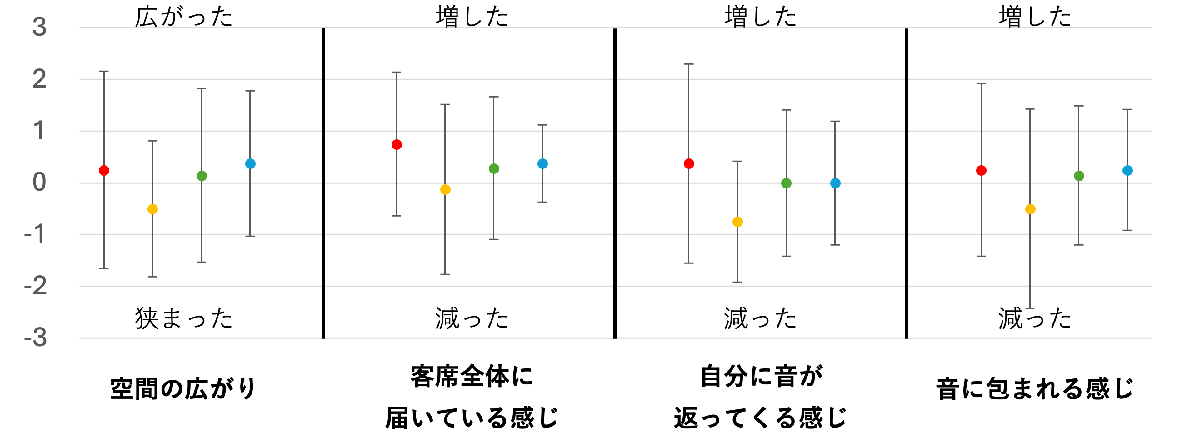
\includegraphics[scale=.55]{images/subjectiveExp/statisticAnalysis/part_space_b.pdf}
      \caption*{音場B}
      \label{fig:空間の印象B}
    \end{minipage}
    \\
    \vspace{1\baselineskip}
    \begin{minipage}{1\linewidth}
      \centering
      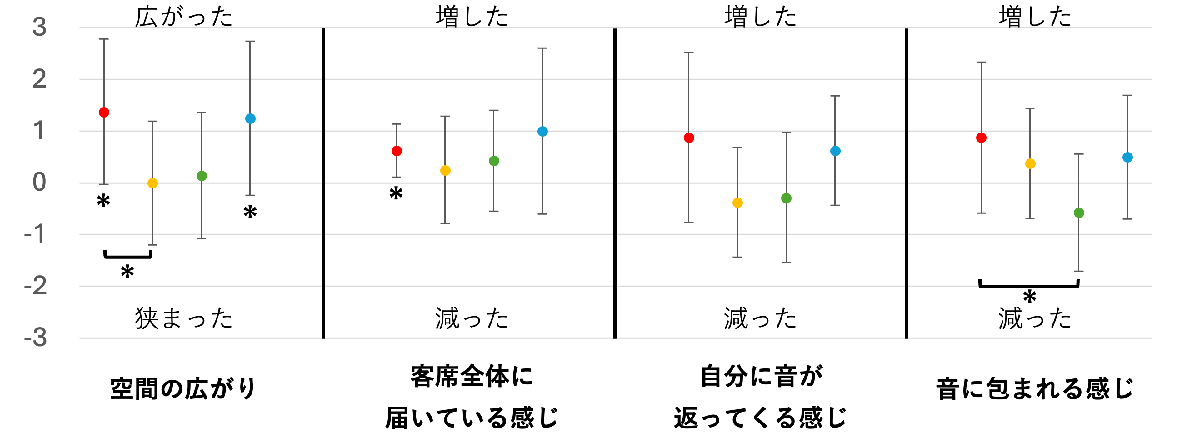
\includegraphics[scale=.55]{images/subjectiveExp/statisticAnalysis/part_space_c.pdf}
      \caption*{音場C}
      \label{fig:空間の印象C}
    \end{minipage}
    \\
    \vspace{1\baselineskip}
    \begin{minipage}{1\linewidth}
      \centering
      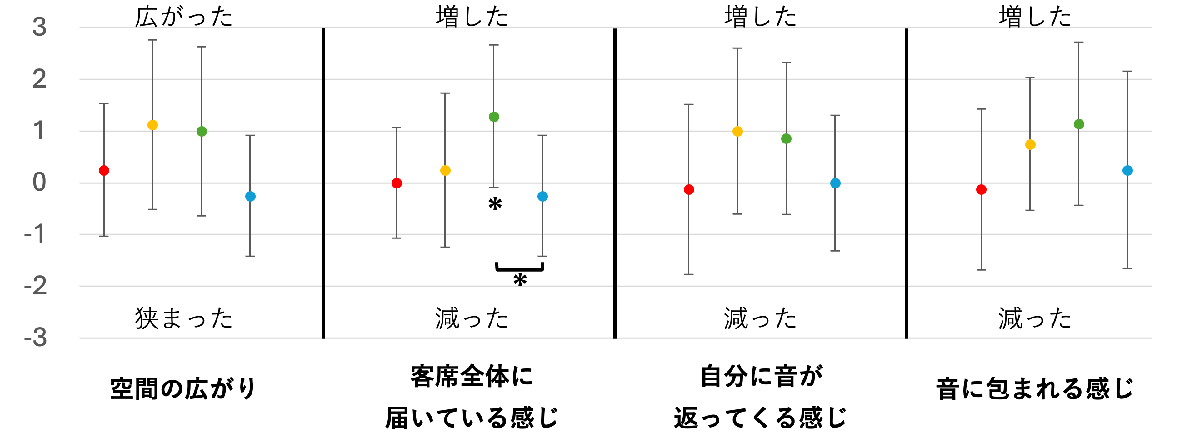
\includegraphics[scale=.55]{images/subjectiveExp/statisticAnalysis/part_space_d.pdf}
      \caption*{音場D}
      \label{fig:空間の印象D}
    \end{minipage}
    
    \caption{パートごとの空間の印象に関する評価}
    \label{fig:パートごとの空間の印象に関する評価}
  \end{figure}


  \newpage
  \begin{figure}[H]
    \centering
    
    \begin{minipage}{1\linewidth}
      \centering
      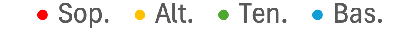
\includegraphics[scale=.55]{images/subjectiveExp/statisticAnalysis/part_legend.pdf}
    \end{minipage}
    \vspace{.5\baselineskip}

    \begin{minipage}{1\linewidth}
      \centering
      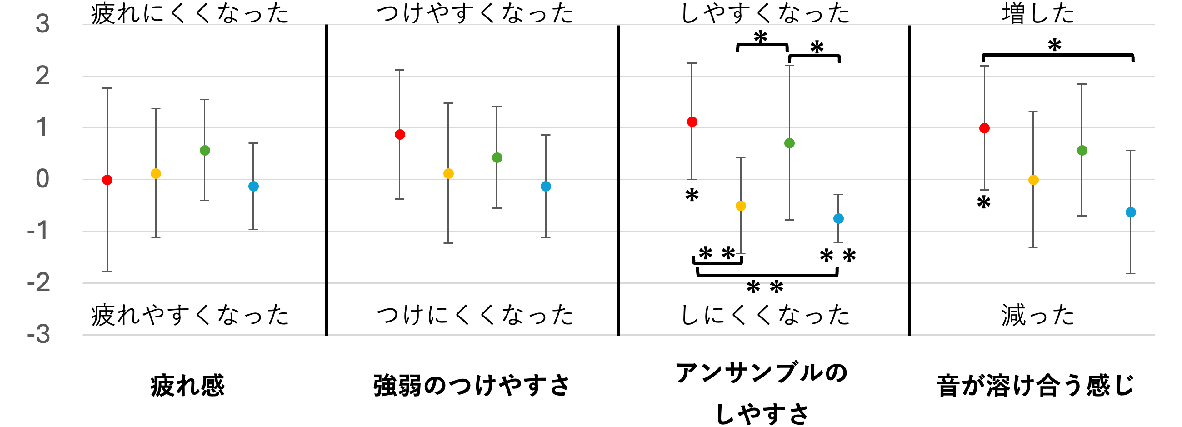
\includegraphics[scale=.55]{images/subjectiveExp/statisticAnalysis/part_performance_a.pdf}
      \caption*{音場A}
      \label{fig:演奏の印象A}
    \end{minipage}
    \\
    \vspace{1\baselineskip}
    \begin{minipage}{1\linewidth}
      \centering
      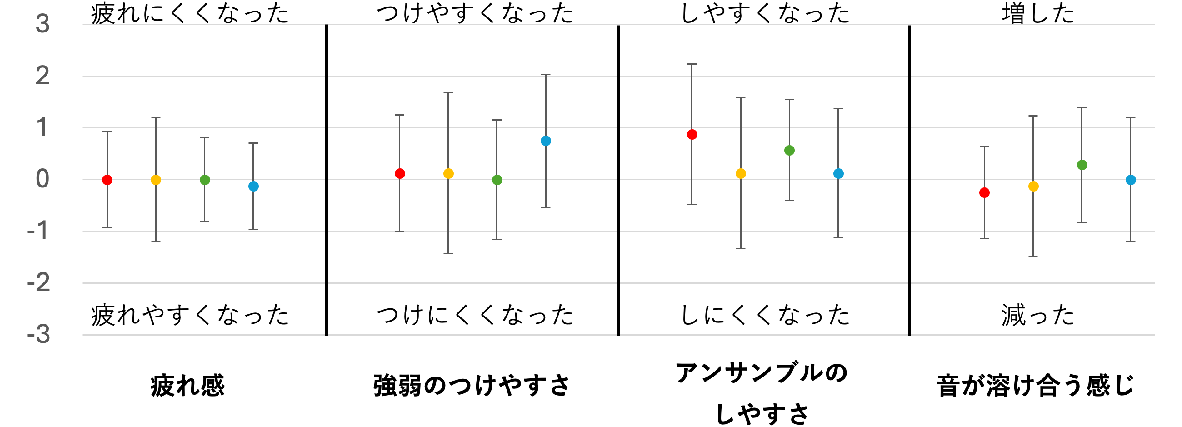
\includegraphics[scale=.55]{images/subjectiveExp/statisticAnalysis/part_performance_b.pdf}
      \caption*{音場B}
      \label{fig:演奏の印象B}
    \end{minipage}
    \\
    \vspace{1\baselineskip}
    \begin{minipage}{1\linewidth}
      \centering
      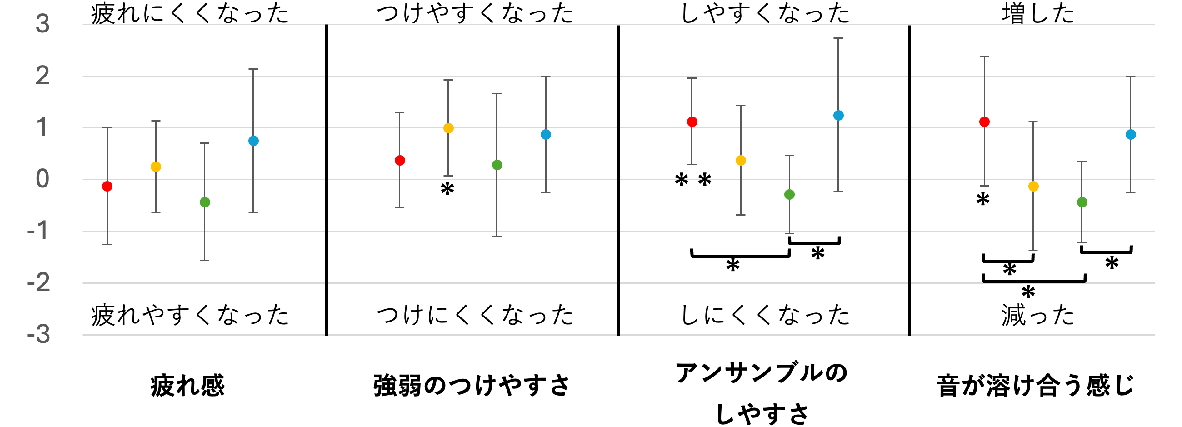
\includegraphics[scale=.55]{images/subjectiveExp/statisticAnalysis/part_performance_c.pdf}
      \caption*{音場C}
      \label{fig:演奏の印象C}
    \end{minipage}
    \\
    \vspace{1\baselineskip}
    \begin{minipage}{1\linewidth}
      \centering
      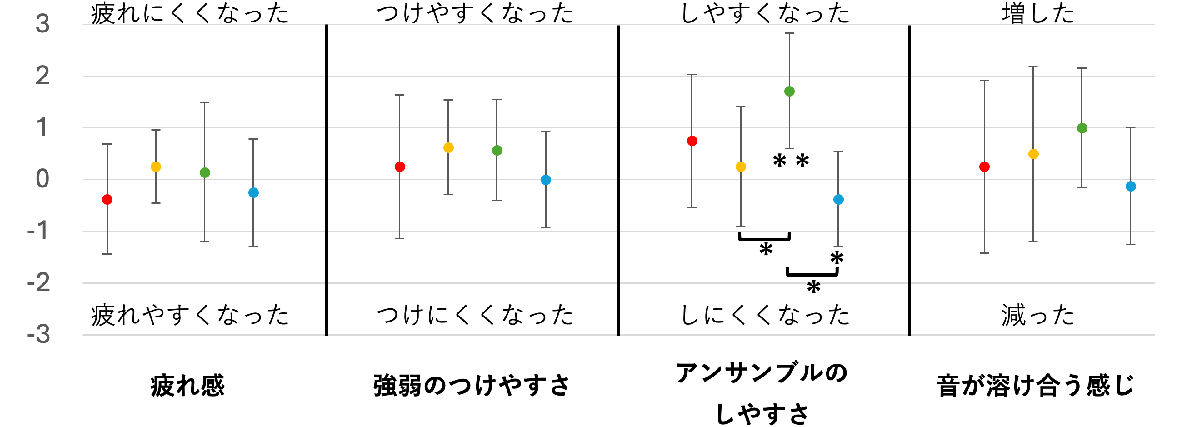
\includegraphics[scale=.55]{images/subjectiveExp/statisticAnalysis/part_performance_d.pdf}
      \caption*{音場D}
      \label{fig:演奏の印象D}
    \end{minipage}
    
    \caption{パートごとの演奏の印象に関する評価}
    \label{fig:パートごとの演奏の印象に関する評価}
  \end{figure}



  \clearpage
  \subsubsection*{総合的な評価}
  なんとかかんとか

  パートごとの総合的な評価について

  パートごとの総合的な評価について

  パートごとの総合的な評価について

  パートごとの総合的な評価について

  パートごとの総合的な評価について

  パートごとの総合的な評価について

  パートごとの総合的な評価について

  パートごとの総合的な評価について

  パートごとの総合的な評価について

  パートごとの総合的な評価について

  パートごとの総合的な評価について

  
  \begin{figure}[H]
    \centering
    
    \begin{minipage}{1\linewidth}
      \centering
      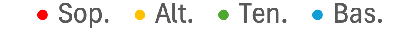
\includegraphics[scale=.55]{images/subjectiveExp/statisticAnalysis/part_legend.pdf}
    \end{minipage}

    \vspace{.5\baselineskip}

    \begin{minipage}{.5\linewidth}
      \centering
      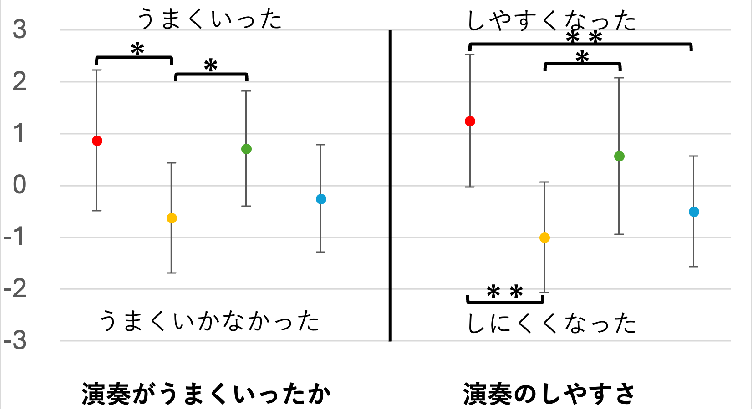
\includegraphics[scale=.55]{images/subjectiveExp/statisticAnalysis/part_overall_a.pdf}
      \caption*{音場A}
      \label{fig:総合的な評価A}
    \end{minipage}%
    \begin{minipage}{.5\linewidth}
      \centering
      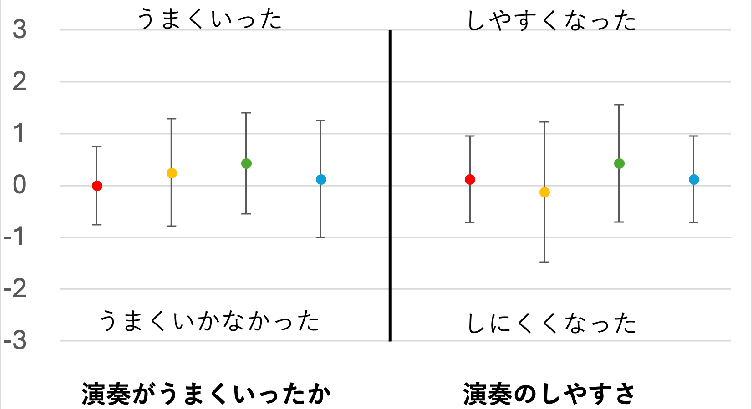
\includegraphics[scale=.55]{images/subjectiveExp/statisticAnalysis/part_overall_b.pdf}
      \caption*{音場B}
      \label{fig:総合的な評価B}
    \end{minipage}

    \vspace{1\baselineskip}

    \begin{minipage}{.5\linewidth}
      \centering
      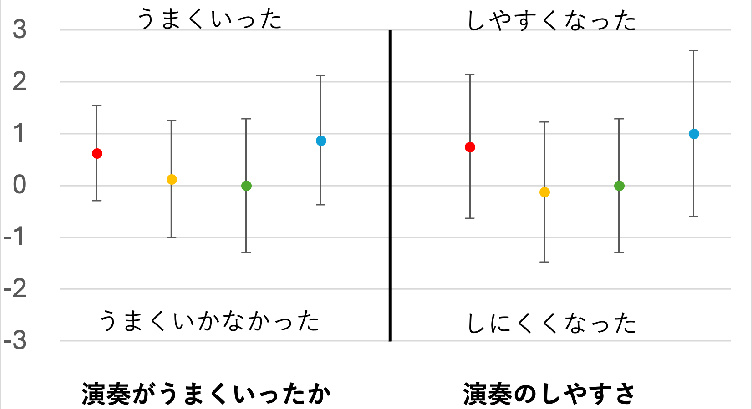
\includegraphics[scale=.55]{images/subjectiveExp/statisticAnalysis/part_overall_c.pdf}
      \caption*{音場C}
      \label{fig:総合的な評価C}
    \end{minipage}%
    \begin{minipage}{.5\linewidth}
      \centering
      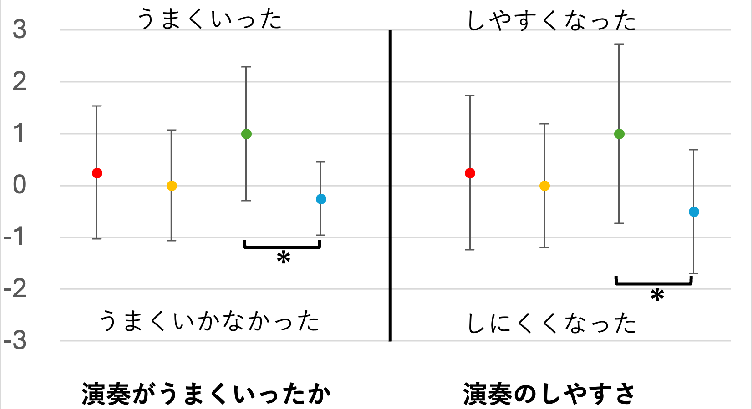
\includegraphics[scale=.55]{images/subjectiveExp/statisticAnalysis/part_overall_d.pdf}
      \caption*{音場D}
      \label{fig:総合的な評価D}
    \end{minipage}
    
    \caption{パートごとの総合的な評価}
    \label{fig:パートごとの総合的な評価}
    
  \end{figure}

  
\clearpage
  全体の傾向として、平均値は1以下と小さい値となった。特に、初期反射音の方向特性に変化を与えた音場Aと音場Bでは
  ほとんどすべての評価項目で0.5以下の値となった。初期反射音は$\SI{0.1}{\second}$以内というごく短い時間に到来する
  ため、主観印象への影響は音色の変化として生じることが多く、大きな音色の変化を伴わない方向特性の変化が
  知覚されにくかったためと考えられる。
  
  また、全体に標準偏差は1以上と大きい値を取っており、これは個人間での音場の評価のばらつきが大きいことを表しているが、
  演奏の印象に関する4項目については標準偏差が比較的小さく、平均値が全体の評価の傾向をあ比較的よく表していると
  考えられる。「疲れ感」の評価については、平均値はほぼ0であり、方向特性による影響はほとんどないと考えられ、
  一方で「強弱のつけやすさ」「アンサンブルのしやすさ」「音が溶け合う感じ」の評価については、後期反射音の前方の反射音を強めた
  音場Cの値が大きい。音場Cは他の評価項目でも比較的高い平均値となっており、前方からの後期反射音の供給によって演奏時の
  印象を向上させることができる可能性があると考えられる。
  
  一方で、響きの印象に関する項目と空間の印象に関する項目について、特に「響きが増えたか」「空間の広がり」「自分に音が返る感じ」
  「音に包まれる感じ」は標準偏差が大きく、平均値が全体の評価の傾向を代表しているとは言えない。これらの評価項目について、
  全被験者の回答の散布図を図\ref{fig:響きが増えたかの散布図}から\ref{fig:音に包まれる感じの散布図}に示す。図中の破線は
  各評価項目について-2または-3を低評価、-1から1を中間評価、2または3を高評価としたときの、評価に応じた被験者の組を示している。
  
  「響きが増えたか」「空間の広がり」「自分に音が返る感じ」「音に包まれる感じ」の評価項目の被験者の分布について、初期反射音に
  方向特性に変化を与えた音場Aと音場Bでは、どちらの評価も低評価から高評価まで広く散らばっているのに対し、後期反射音に方向特性を与えた音場Cと
  音場Dの分布では、少なくとも一方を高く評価した被験者が多い傾向が見られる。このことから、後期反射音の方向特性に変化を与えることで、
  響きの印象や空間の印象を向上させることができる可能性があることが示唆される。

  \begin{figure}[H]
    \centering
    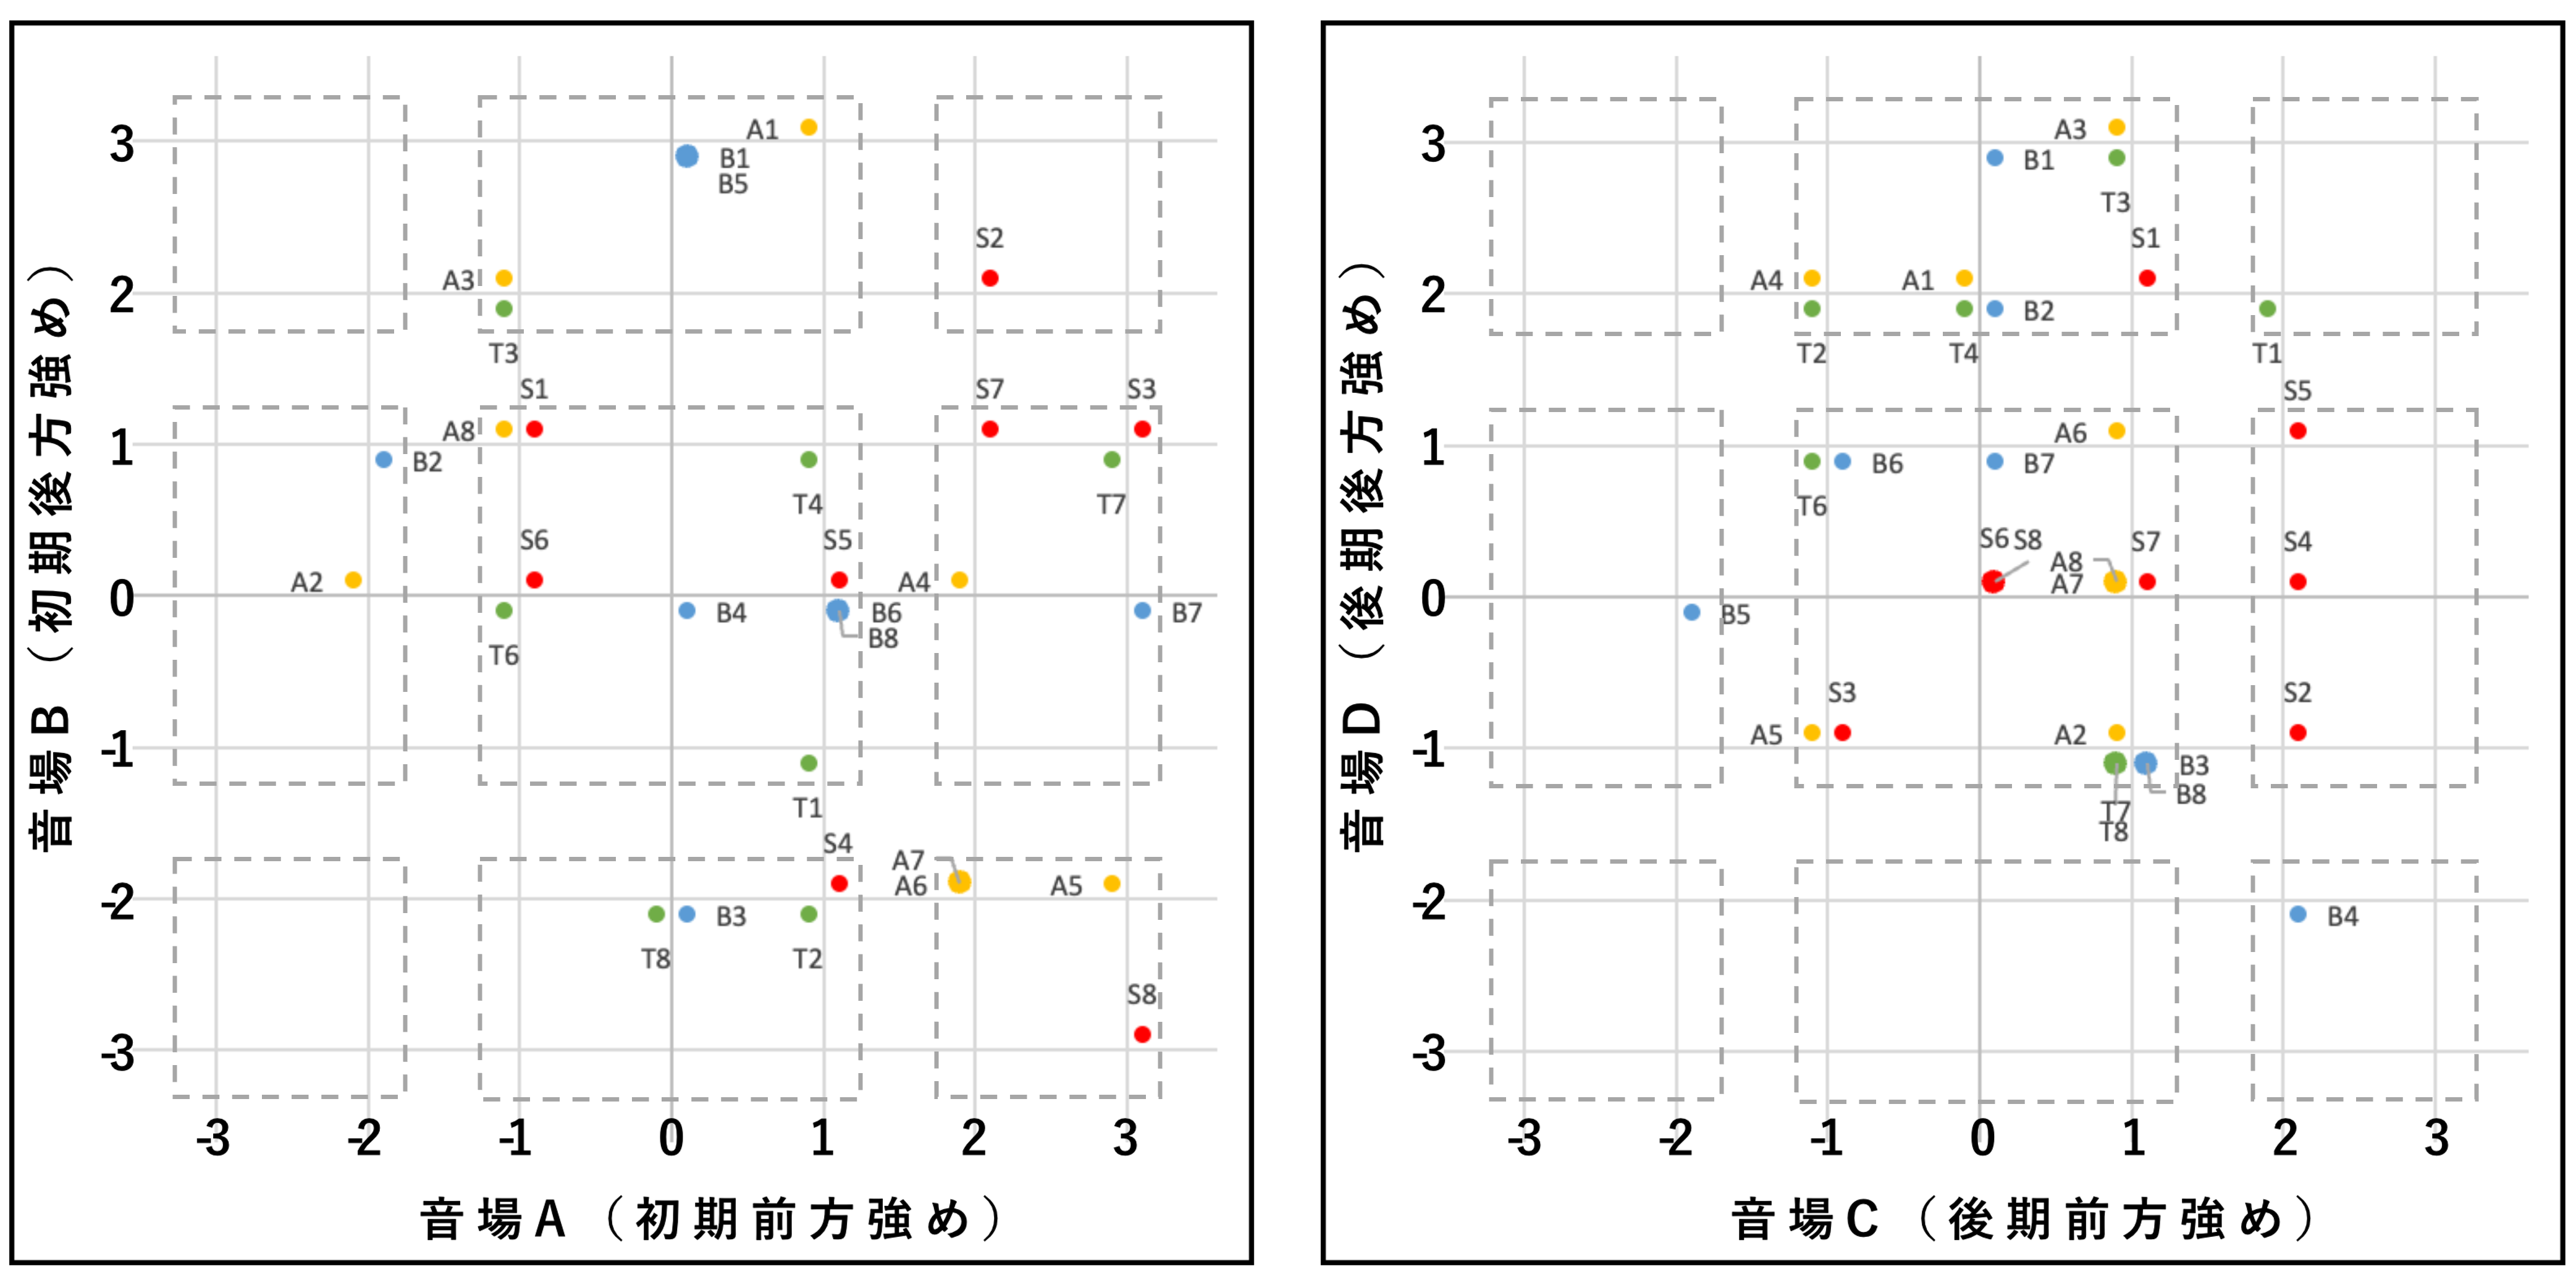
\includegraphics[width=1\linewidth]{images/subjectiveExp/scat01reverb.png}
    \caption{響きが増えたか}
    \label{fig:響きが増えたかの散布図}
  \end{figure}

  \begin{figure}[H]
    \centering
    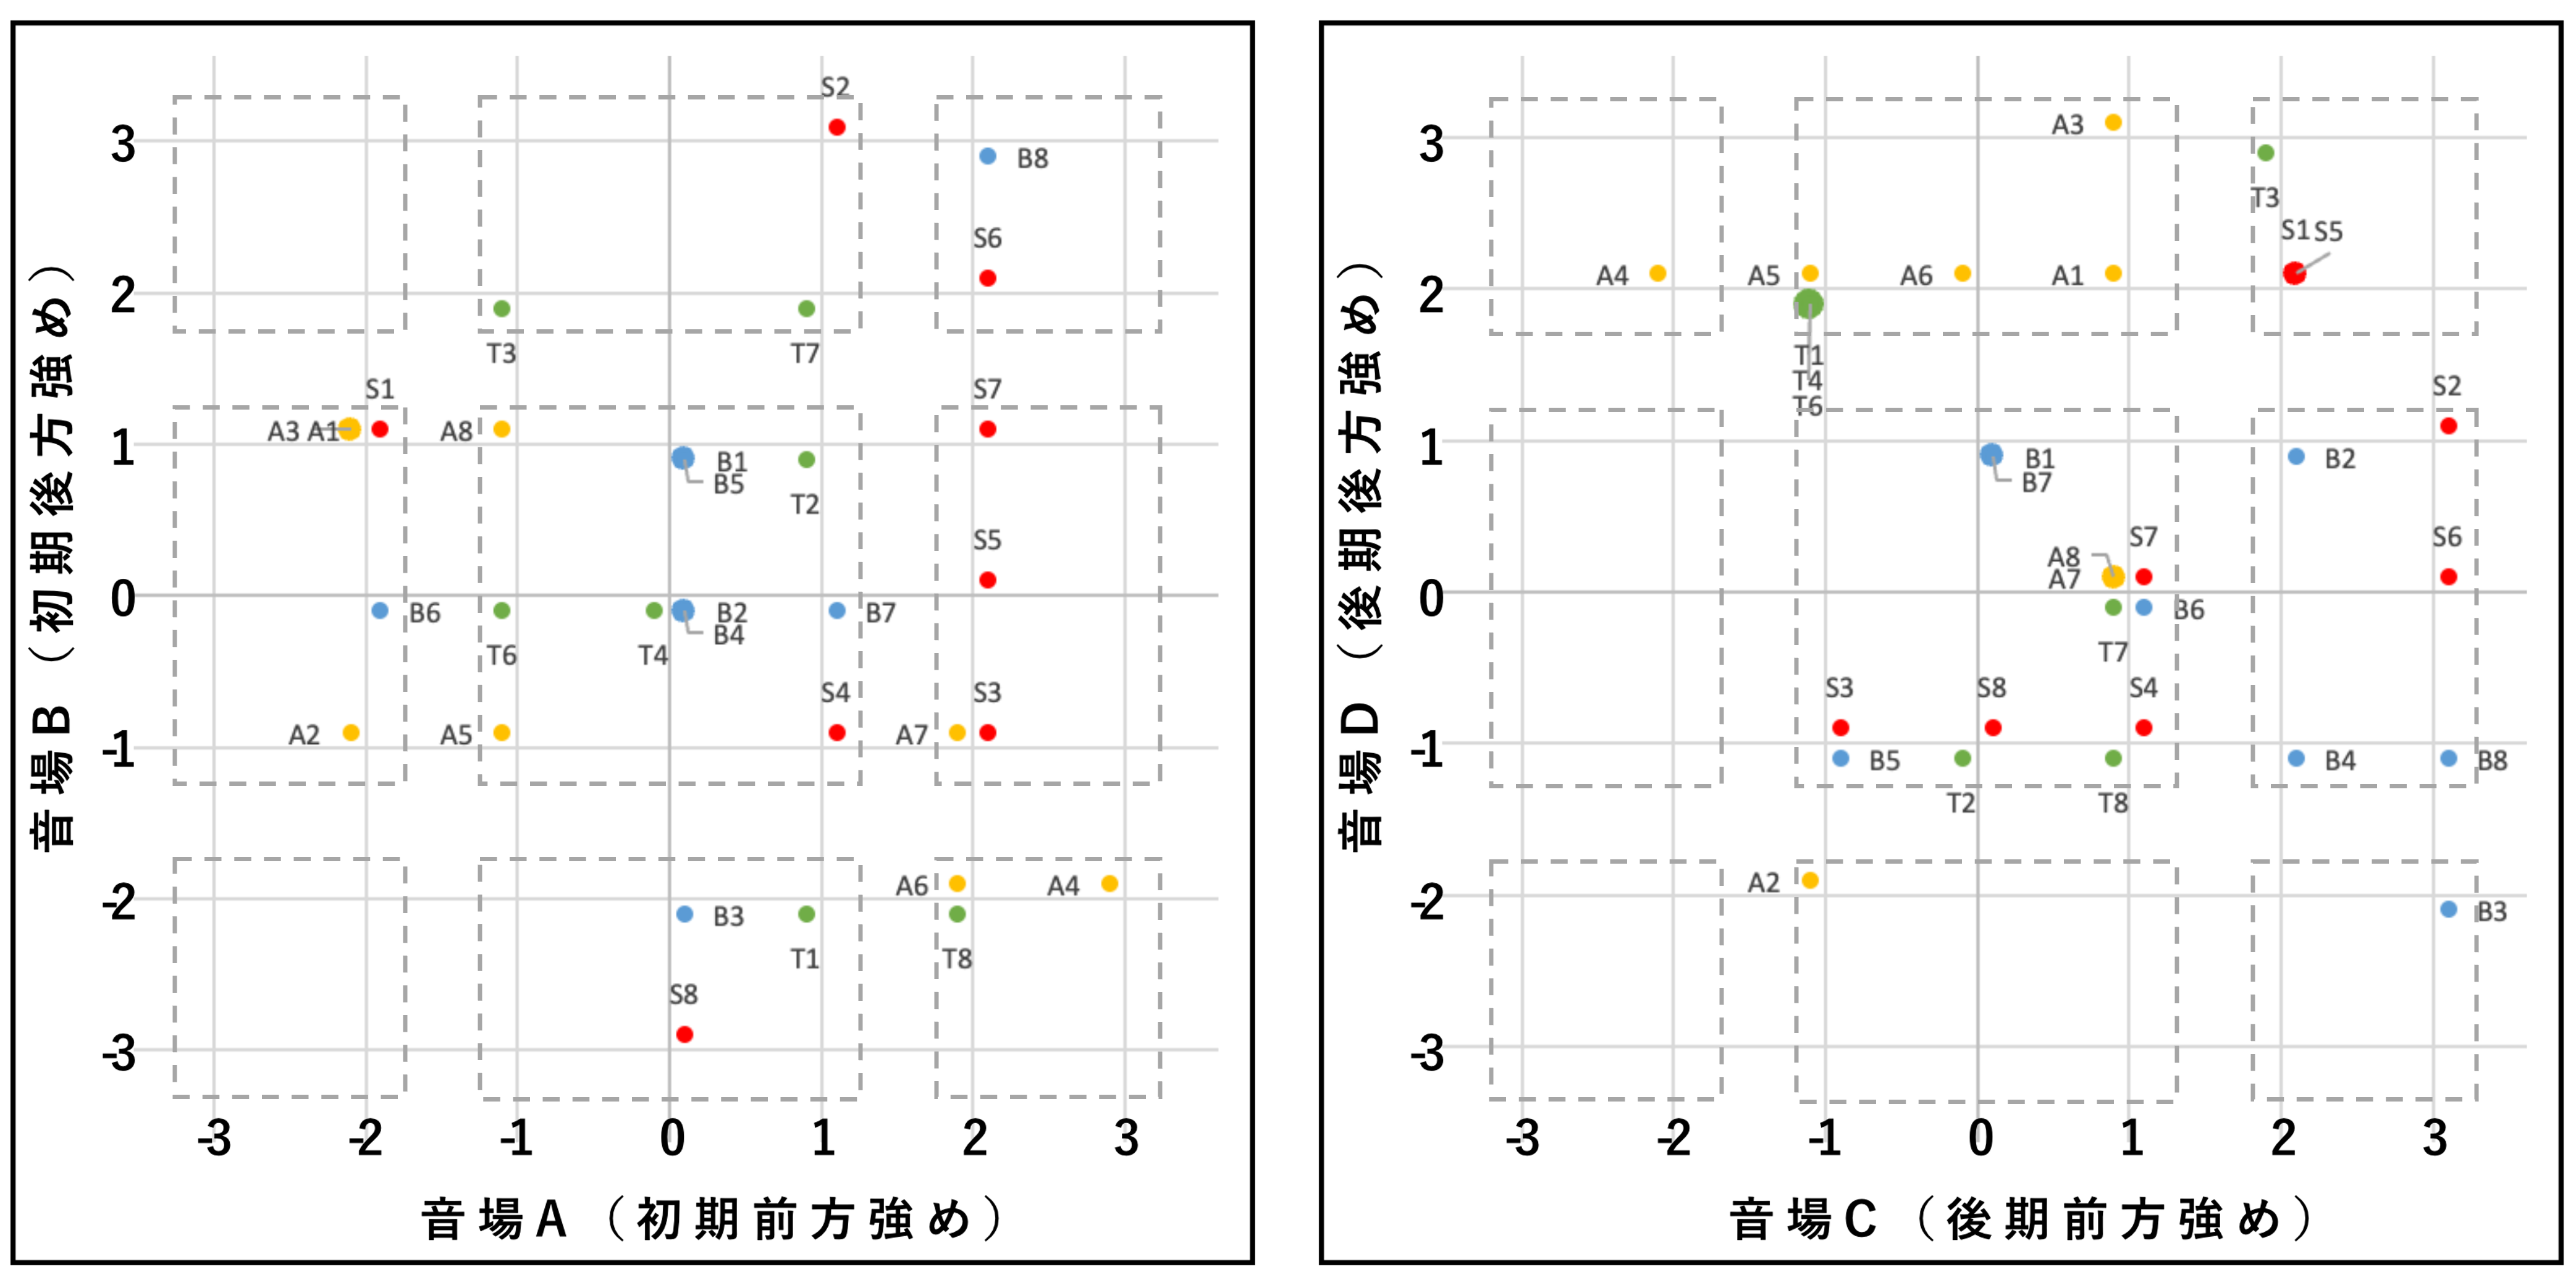
\includegraphics[width=1\linewidth]{images/subjectiveExp/scat04spacy.png}
    \caption{空間の広がり}
    \label{fig:空間の広がりの散布図}
  \end{figure}

  \begin{figure}[H]
    \centering
    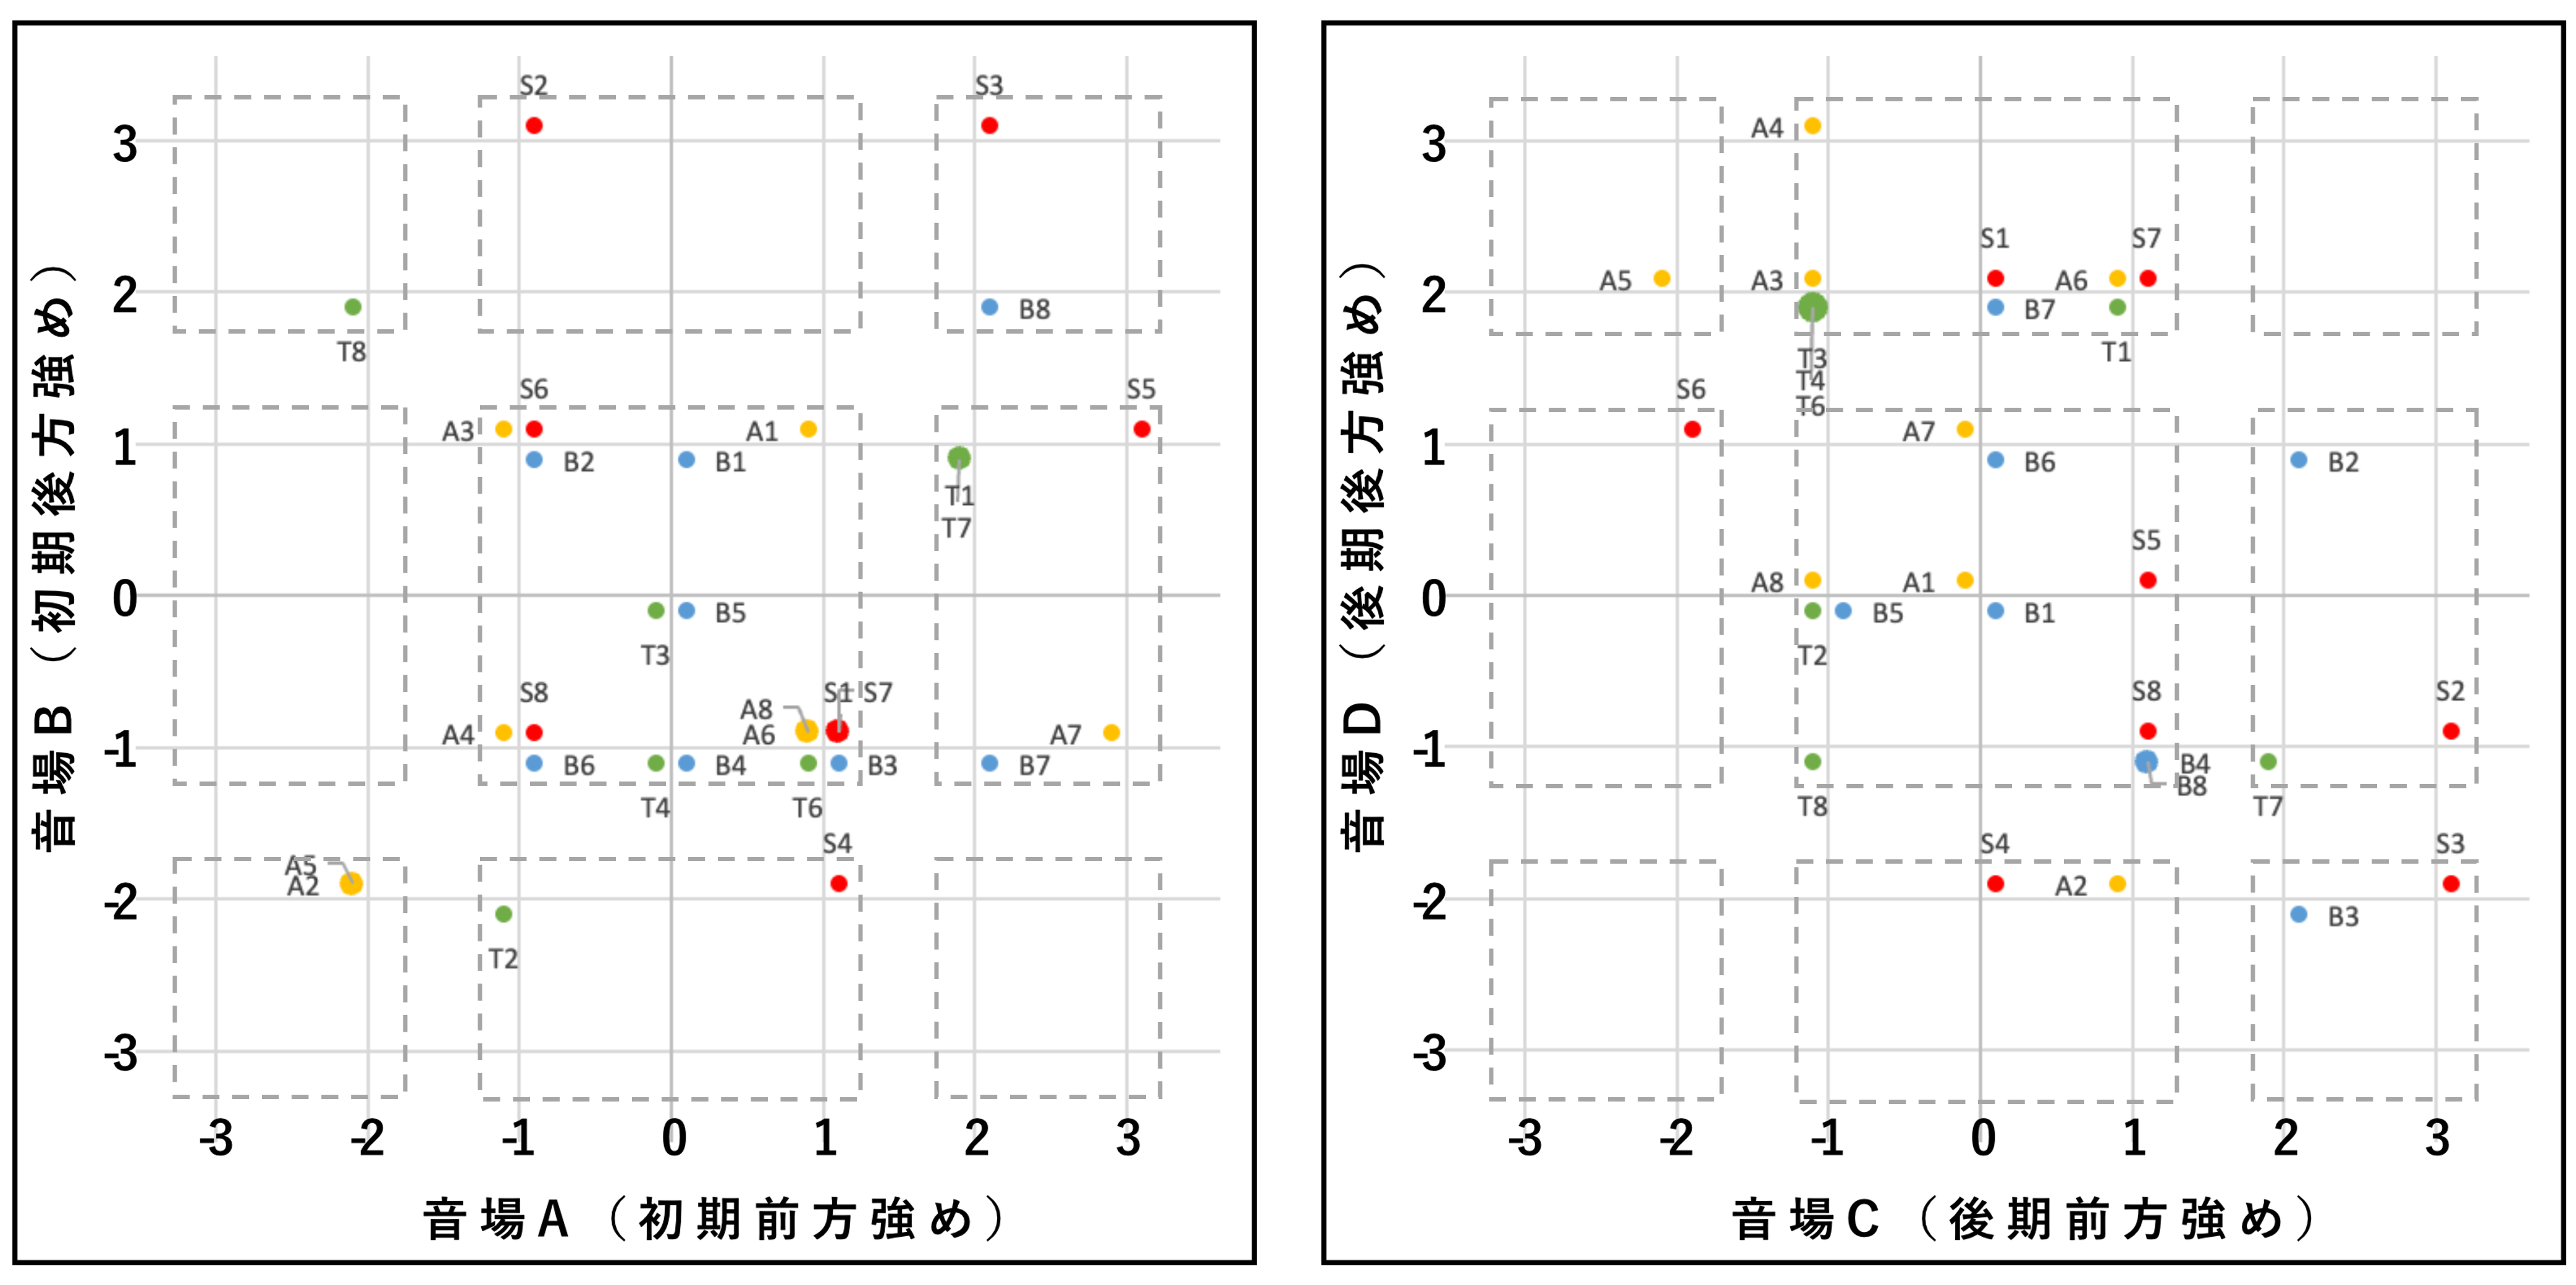
\includegraphics[width=1\linewidth]{images/subjectiveExp/scat06returnSelf.png}
    \caption{自分に音が返る感じ}
    \label{fig:自分に音が返る感じの散布図}
  \end{figure}

  \begin{figure}[H]
    \centering
    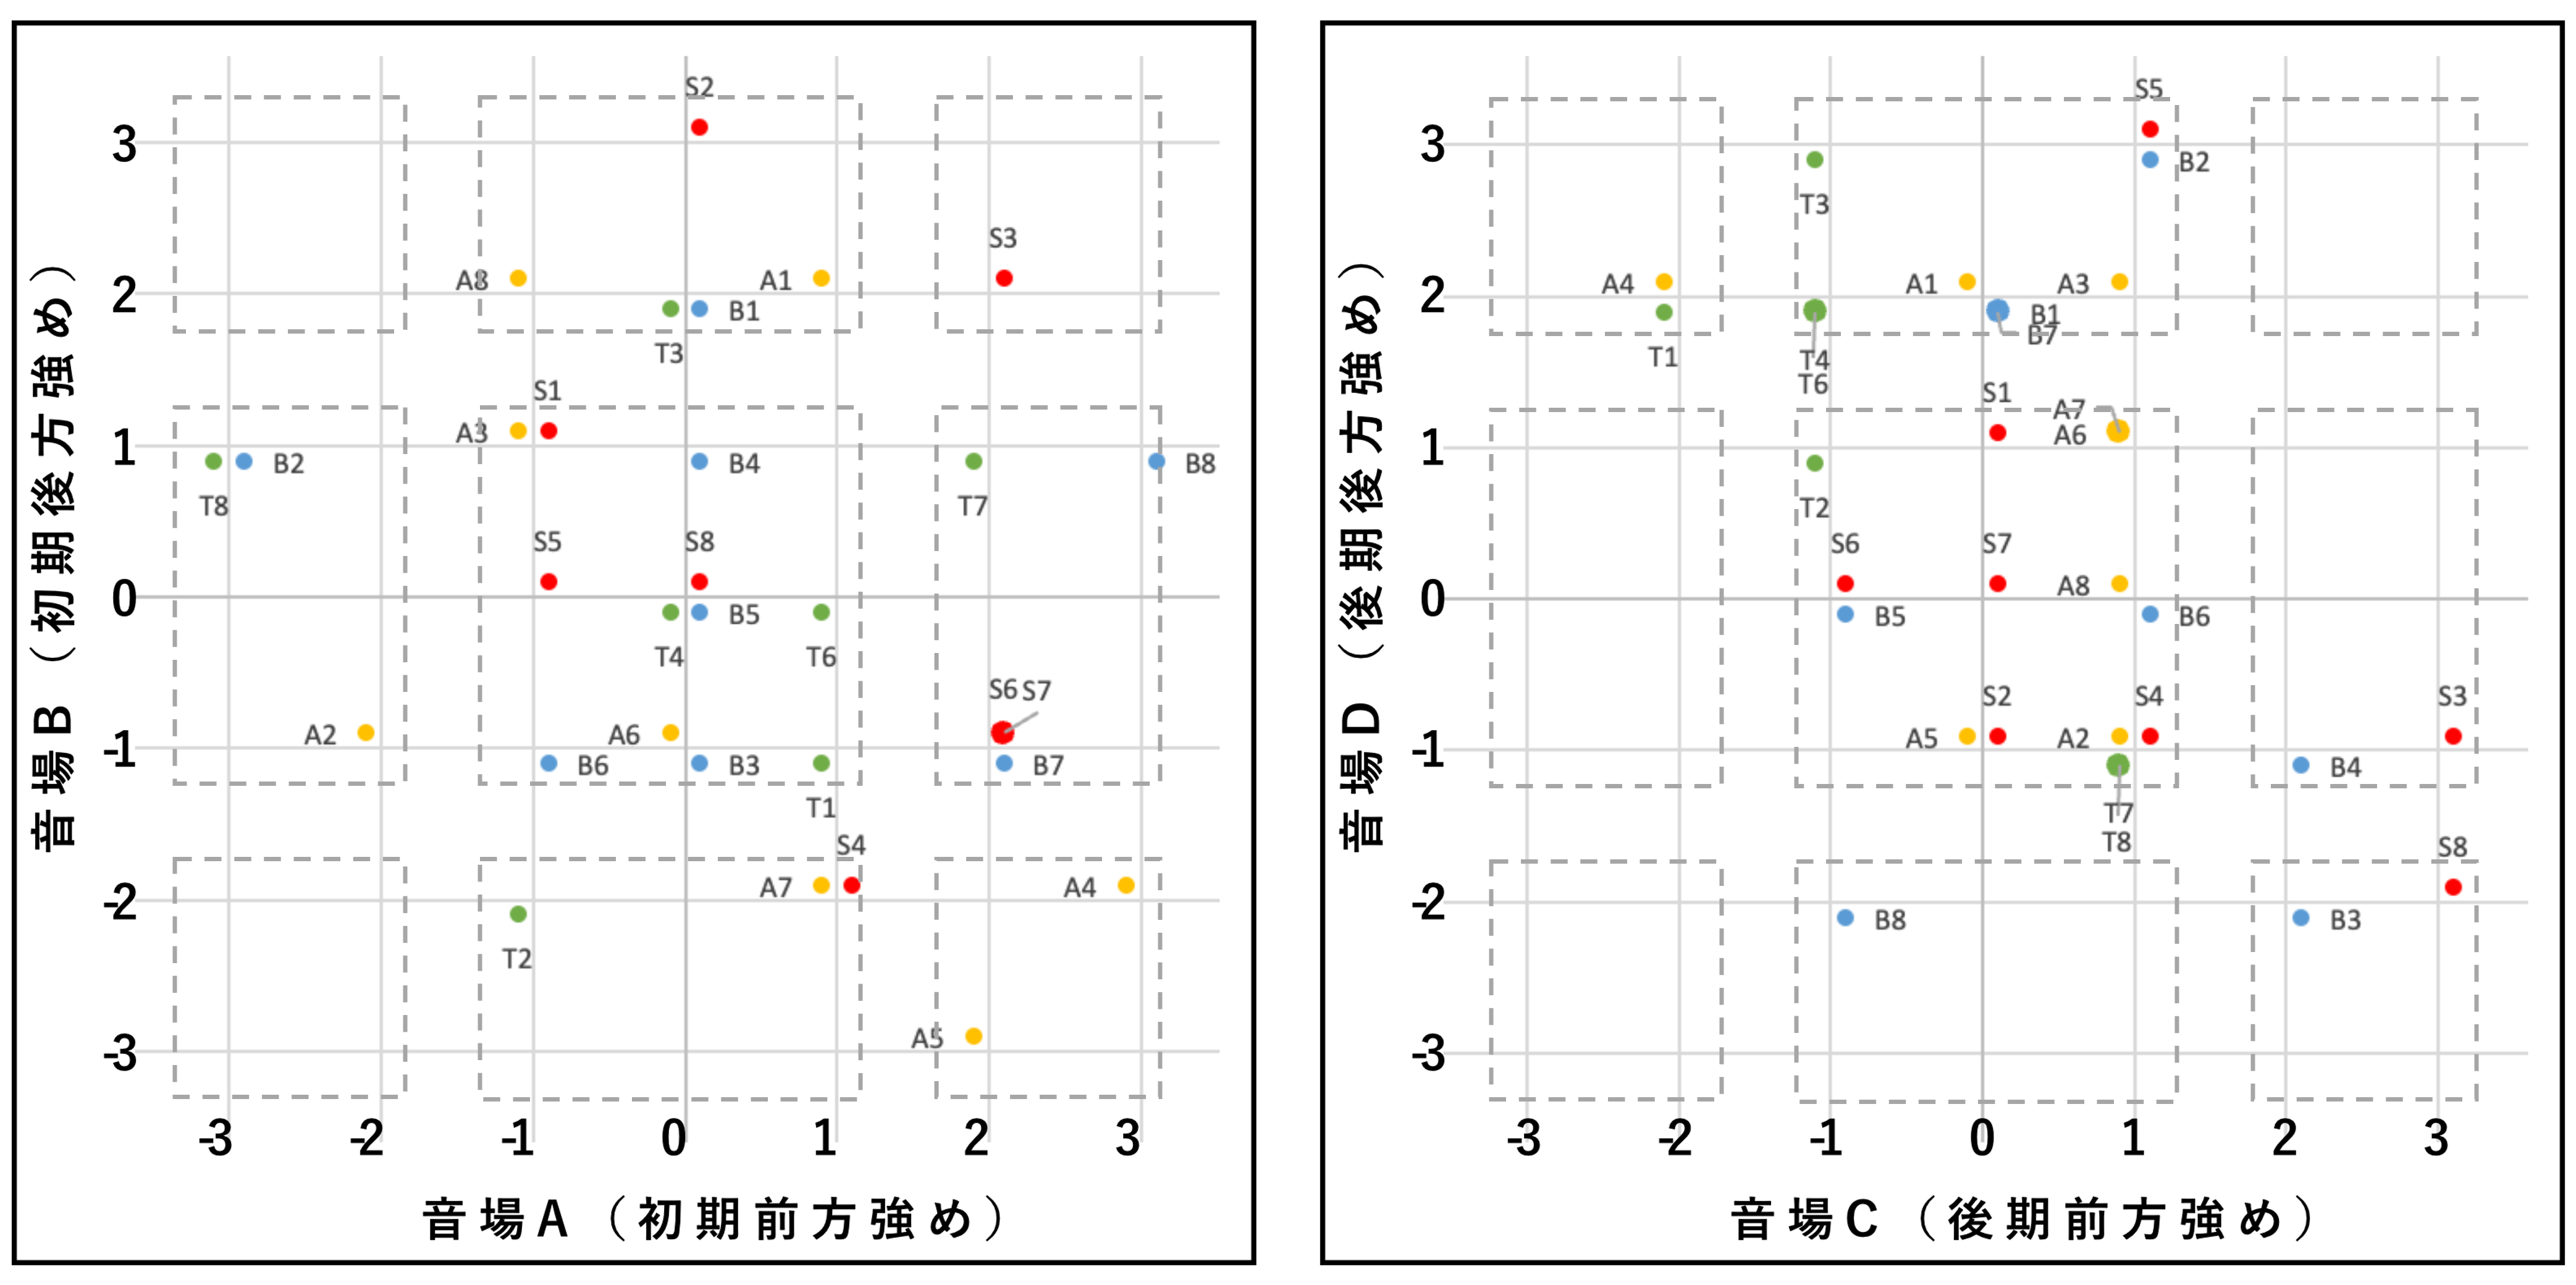
\includegraphics[width=1\linewidth]{images/subjectiveExp/scat07surrounded.png}
    \caption{音に包まれる感じ}
    \label{fig:音に包まれる感じの散布図}
  \end{figure}

%=====================================================================================

\clearpage
\begin{table}[H]
  \centering
  \begin{adjustbox}{width=.6\linewidth}
    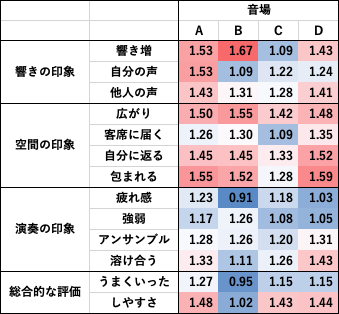
\includegraphics{images/subjectiveExp/subjectiveStd.png}
  \end{adjustbox}
  \caption{表のキャプション}
  \label{table:1}
\end{table}

% 参考文献
% 参考文献の箇所にインプットしてください。

% 分割ファイル内でのみ,bibliographyを読み込みます。

\expandafter\ifx\csname ifdraft\endcsname\relax

  % bibliographyを展開する

  \bibliographystyle{junsrt}
  \bibliography{ref.bib}% 同じディレクトリ内のbibファイルのみを参照可能

\fi

\end{document}